\documentclass{beamer}

%\usetheme{Madrid}
%\usetheme{Boadilla}
%\usetheme{default}
%\usetheme{Warsaw}
%\usetheme{Bergen}
%\usetheme{Frankfurt}
\usetheme{Darmstadt}

\setbeamercolor{normal text}{fg=white}
\setbeamertemplate{background canvas}[vertical shading] [top=black!95,bottom=black!65]

\definecolor{mypurple}{RGB}{207,78,64}
\usecolortheme[named=mypurple]{structure}

\definecolor{myorange}{RGB}{255,235,190}
\beamerboxesdeclarecolorscheme{orange}{orange}{myorange}

\definecolor{commandcolor}{RGB}{111,195,165}

\setbeamertemplate{footline}[page number]
%\setbeamercovered{transparent}
\setbeamercovered{invisible}
\setbeamertemplate{navigation symbols}{}

%\usepackage{musixtex}
\usepackage{multimedia}
\usepackage{graphicx}
\usepackage[utf8]{inputenc}
%\usepackage[T1]{fontenc}
\usepackage[french]{babel} 
%\usepackage[all]{xy}
%\usepackage{multirow}
%\usepackage{lmodern}
\usepackage{subfigure}
%\usepackage{ulem}
\usepackage{url}
\usepackage{hyperref}
\usepackage{verbatim}
\usepackage{xspace}
\usepackage{color}
\usepackage{xcolor}
\usepackage{rotating}
\usepackage{multicol}
\usepackage[export]{adjustbox}
\usepackage{textpos}
\usepackage{listings}
\usepackage{fontawesome}


\definecolor{mypurple}{RGB}{207,78,64}
\usecolortheme[named=mypurple]{structure}

\definecolor{myorange}{RGB}{255,235,190}
\beamerboxesdeclarecolorscheme{orange}{orange}{myorange}

\definecolor{dgreen}{RGB}{0,125,0}

\usepackage{tikz}
\usetikzlibrary{trees}

\setbeamertemplate{caption}[numbered] 

\newcommand{\setframetitle}[1]{\begin{center}
    \huge \textbf{#1}
\end{center}}


%% --------------

\title{Docker}
\subtitle{Atelier d'aide à la programmation}
\author{L\'eo \textsc{Baudouin}}
\institute{
  {\url{baudouin.leo @ gmail.com}}
}
\date{19-20 juin 2025}

%% --------------

\begin{document}

\begin{frame}
  \titlepage
\end{frame}

\section{Introduction}
\subsection{}

\begin{frame}{Définition}


\begin{center}

\includegraphics[width=0.5\linewidth]{images/docker-logo}
\end{center}

\begin{block}{Wikipedia}
{\it 
«~Docker est un outil qui peut empaqueter une application et ses dépendances dans un conteneur isolé, qui pourra être exécuté sur n'importe quel serveur~».

Ceci permet d'étendre la flexibilité et la portabilité d’exécution d'une application, que ce soit sur la machine locale, un cloud privé ou public, une machine nue...}
\end{block}
\end{frame}


\begin{frame}[fragile]{Installer Docker}

\begin{block}{Installer et configurer}
\textcolor{cyan}{\verb?sudo apt-get install -y docker.io?}

\textcolor{cyan}{\verb?sudo groupadd docker?}

\textcolor{cyan}{\verb?sudo usermod -aG docker \$USER?}
\end{block}

\begin{block}{Docker for Windows}
\href{https://docs.docker.com/docker-for-windows/install/}{https://docs.docker.com/docker-for-windows/install/}
\end{block}

\end{frame}


\begin{frame}{Démarrer un conteneur}

\begin{block}{Télécharger une image}
\textcolor{cyan}{\verb?docker pull ubuntu:18.04?}
\end{block}

\begin{block}{Démarrer un conteneur}
\textcolor{cyan}{\verb?docker run --rm -it ubuntu:18.04?}
\end{block}

\end{frame}

\section{Images}
\subsection{Création}

\begin{frame}[fragile]{Créer une image pour \LaTeX}
\begin{block}{Dockerfile}
\begin{verbatim}
FROM ubuntu:18.04

RUN apt-get update
RUN apt-get upgrade -y 
RUN apt-get install -y texlive-full
\end{verbatim}
\end{block}
\end{frame}

\begin{frame}[fragile]{Créer une image pour Angular}
\begin{block}{Dockerfile}
\scriptsize
\begin{verbatim}
FROM ubuntu:18.04

RUN apt-get update && apt-get -y upgrade
RUN apt-get install -y npm

RUN npm install -g npm@latest
RUN npm install -g @angular/cli
RUN npm install --save-dev @angular-devkit/build-angular
RUN npm install --save-dev @angular/compiler-cli
RUN npm install --save-dev @angular/compiler
WORKDIR /sources

EXPOSE 8082
EXPOSE 4200

# ng serve --host 0.0.0.0
\end{verbatim}
\end{block}
\end{frame}



\begin{frame}[fragile]{Créer une image avec une interface}
\begin{block}{Dockerfile}
\scriptsize
\begin{verbatim}
FROM ubuntu:16.04

RUN apt-get update
RUN apt-get install -y x-window-system
RUN apt-get install -y binutils
RUN apt-get install -y mesa-utils
RUN apt-get install -y module-init-tools

ADD nvidia-driver.run /tmp/nvidia-driver.run
RUN sh /tmp/nvidia-driver.run -a -N --ui=none --no-kernel-module
RUN rm /tmp/nvidia-driver.run

RUN apt-get install -y nano

CMD /bin/bash

WORKDIR /sources
\end{verbatim}
\end{block}
\end{frame}



\section{Compose}
\subsection{}

\begin{frame}{docker-compose}
\begin{block}{Wikipedia}
{\it 
Docker \textbf{compose} est un outil très intéressant de gestion de package docker. Cet outil va lancer vos conteneurs et leurs éventuels liens à partir d'un fichier de configuration écrit en yaml.}
\end{block}
\end{frame}

\begin{frame}[fragile]{}
\begin{block}{\tiny docker-compose.yml}
\tiny
\begin{verbatim}
version: '3.3'
services:
   db:
     image: mysql:5.7
     volumes:
       - db_data:/var/lib/mysql
     restart: always
     environment:
       MYSQL_ROOT_PASSWORD: somewordpress
       MYSQL_DATABASE: wordpress
       MYSQL_USER: wordpress
       MYSQL_PASSWORD: wordpress
   wordpress:
     depends_on:
       - db
     image: wordpress:latest
     ports:
       - "8000:80"
     restart: always
     environment:
       WORDPRESS_DB_HOST: db:3306
       WORDPRESS_DB_USER: wordpress
       WORDPRESS_DB_PASSWORD: wordpress
   adminer:
     image: adminer
     depends_on:
       - db
     ports:
       - "8080:8080"
     restart: always
volumes:
    db_data:
\end{verbatim}
\end{block}
\end{frame}

\begin{frame}[fragile]{Démarrer / Arrêter}
\begin{block}{Gestion}
\textcolor{cyan}{\verb?docker-compose up [-d]?}

\textbf{-d} = run containers in the background
\newline

\textcolor{cyan}{\verb?docker-compose down?}
\end{block}
\end{frame}


\section{UI}
\subsection{}

\begin{frame}[fragile]{Gérer ses dockers}
\begin{block}{CLI}
\textcolor{cyan}{\verb?docker ps [-a]?}

\textcolor{cyan}{\verb?docker images?}
\end{block}

\begin{block}{Portainer}
\textcolor{cyan}{\verb?docker volume create portainer\_data?}

\textcolor{cyan}{\verb?docker run -d -p 9000:9000 --restart always -v /var/run/docker.sock:/var/run/docker.sock -v portainer\_data:/data portainer/portainer?}
\end{block}
\end{frame}


\begin{frame}[fragile]{Gérer ses dockers}
\begin{block}{Portainer}
\begin{center}
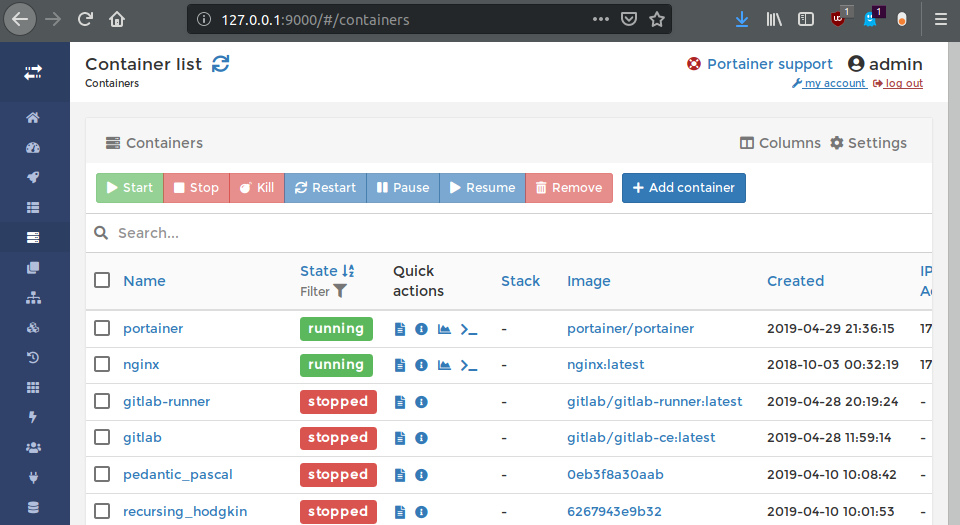
\includegraphics[width=1.0\linewidth]{images/portainer}
\end{center}
\end{block}
\end{frame}

\section{Créer une image Docker}

\subsection{Commandes}

\begin{frame}[fragile]{Commandes Docker utiles}
\begin{block}{Gestion des images}
\textcolor{cyan}{\verb?docker images?} : Liste les images disponibles \\
\textcolor{cyan}{\verb?docker pull <image>?} : Télécharge une image \\
\textcolor{cyan}{\verb?docker rmi <image>?} : Supprime une image
\end{block}

\begin{block}{Gestion des conteneurs}
\textcolor{cyan}{\verb?docker ps?} : Liste les conteneurs actifs \\
\textcolor{cyan}{\verb?docker ps -a?} : Liste tous les conteneurs \\
\textcolor{cyan}{\verb?docker run <image>?} : Lance un conteneur \\
\textcolor{cyan}{\verb?docker stop <container>?} : Arrête un conteneur \\
\textcolor{cyan}{\verb?docker rm <container>?} : Supprime un conteneur
\end{block}
\end{frame}


\begin{frame}[fragile]{Commandes Docker utiles}

\begin{block}{Autres commandes utiles}
\textcolor{cyan}{\verb?docker exec -it <container> bash?} : Accès shell dans un conteneur \\
\textcolor{cyan}{\verb?docker logs <container>?} : Affiche les logs d'un conteneur \\
\textcolor{cyan}{\verb?docker tag <image>:<tag> <repository>/<image>:<tag>?} : Taguer une image pour un dépôt distant \\
\textcolor{cyan}{\verb?docker push <repository>/<image>:<tag>?} : Pousser une image vers un registre distant \\
\end{block}


\begin{block}{Build commands}
\textcolor{cyan}{\verb?docker build -t <image>:<tag> .?} : Construit une image à partir du Dockerfile dans le répertoire courant \\
\textcolor{cyan}{\verb?docker build -f <Dockerfile> -t <image>:<tag> .?} : Spécifie un Dockerfile différent\\
\end{block}

\end{frame}


\begin{frame}[fragile]{Commandes Docker utiles}
\begin{block}{Exemples d'utilisation de \texttt{docker run}}
\textcolor{cyan}{\verb?docker run hello-world?} : Teste l'installation de Docker \\
\textcolor{cyan}{\verb?docker run -it ubuntu:latest bash?} : Lance un shell interactif dans un conteneur Ubuntu \\
\textcolor{cyan}{\verb?docker run -d -p 8080:80 nginx?} : Démarre Nginx en arrière-plan et mappe le port 80 du conteneur sur le port 8080 de l'hôte \\
\textcolor{cyan}{\verb?docker run --name monconteneur alpine echo "Bonjour"?} : Donne un nom au conteneur et exécute une commande simple \\
\textcolor{cyan}{\verb?docker run -v \$(pwd):/data ubuntu ls /data?} : Monte le dossier courant dans le conteneur et liste son contenu \\
\end{block}
\end{frame}


\subsection{Exercice}

\begin{frame}{Exercice 1 : Créer une image Ubuntu personnalisée}
\begin{block}{Objectif}
Créez un \texttt{Dockerfile} qui utilise l'image \texttt{ubuntu:latest} et installe les paquets suivants :
\begin{itemize}
  \item \texttt{curl}
  \item \texttt{git}
\end{itemize}
Construisez l'image et lancez un conteneur pour vérifier que les commandes \texttt{curl} et \texttt{git} sont disponibles.
\end{block}
\end{frame}

\begin{frame}{Exercice 2 : Image Python avec script}
\begin{block}{Objectif}
\begin{itemize}
  \item Créez un \texttt{Dockerfile} basé sur \texttt{python:3.10-slim}.
  \item Copiez un script Python local dans l'image dans un dossier /work.
  \item Configurez le conteneur pour exécuter ce script au démarrage.
  \item Vérifiez que le script s'exécute correctement en lançant le conteneur.
\end{itemize}
\end{block}
\end{frame}

\begin{frame}{Exercice 3 : Serveur Web statique}
\begin{block}{Objectif}
\begin{itemize}
  \item Créez un \texttt{Dockerfile} qui utilise l'image \texttt{nginx:latest}.
  \item Copiez une page HTML personnalisée dans le répertoire de contenu statique de Nginx (dossier /usr/share/nginx/html).
  \item Configurez le conteneur pour exposer le port 80.
  \item Lancez le conteneur en partageant le port 80 et accédez à la page HTML via un navigateur.
\end{itemize}
\end{block}
\end{frame}

\begin{frame}{Exercice 4 : Application Flask simple}
\begin{block}{Objectif}
\begin{itemize}
  \item Créez un \texttt{Dockerfile} pour une application web Python utilisant Flask.
  \item L'application doit afficher "Bonjour Docker" sur le port 5000.
  \item Utilisez l'image de base \texttt{python:3.10-slim}.
  \item Lancez le conteneur et accédez à l'application via un navigateur.
\end{itemize}
\end{block}
\end{frame}

\begin{frame}{Exercice 5 : Persistance des données avec volumes}
\begin{block}{Objectif}
\begin{itemize}
  \item Créez un volume Docker pour persister les données d'une base de données MySQL.
  \item Lancez un conteneur \texttt{mysql:8} en utilisant ce volume.
  \item Vérifiez que les données persistent après l'arrêt et le redémarrage du conteneur.
\end{itemize}
\end{block}
\end{frame}

\begin{frame}{Exercice 6 : Dockeriser une application Java}
\begin{block}{Objectif}
\begin{itemize}
  \item Créez un \texttt{Dockerfile} pour une application Java (fichier \texttt{.jar}).
  \item Utilisez l'image officielle \texttt{openjdk} comme base.
  \item Configurez le conteneur pour exécuter ce fichier \texttt{.jar} au démarrage.
  \item Lancez le conteneur et vérifiez que l'application fonctionne correctement.
\end{itemize}
\end{block}
\end{frame}

\begin{frame}{Exercice 7 : Variables d'environnement et secrets}
\begin{block}{Objectif}
\begin{itemize}
  \item Créez un \texttt{Dockerfile} pour une application Bash simple qui affiche un message.
  \item Configurez le script Bash pour lire une variable d'environnement (par exemple, un message personnalisé).
  \item Lancez le conteneur en passant cette variable d'environnement.
  \item Vérifiez que le script affiche le message personnalisé.
\end{itemize}
\end{block}
\end{frame}

\begin{frame}{Exercice 8 : Limiter les ressources d'un conteneur}
\begin{block}{Objectif}
\begin{itemize}
  \item Créez un conteneur Docker basé sur l'image \texttt{ubuntu:latest}.
  \item Limitez la mémoire du conteneur à 256Mo et le CPU à 0.5.
  \item Vérifiez que ces limites sont bien appliquées en utilisant la commande \texttt{docker stats}.
\end{itemize}
\end{block}
\end{frame}

\begin{frame}{Exercice 9 : Docker et réseau personnalisé}
\begin{block}{Objectif}
\begin{itemize}
  \item Créez un réseau Docker personnalisé.
  \item Lancez deux conteneurs (par exemple, un serveur web et une base de données) sur ce réseau.
  \item Assurez-vous que les conteneurs peuvent communiquer entre eux uniquement via ce réseau.
  \item Utilisez Docker Compose pour orchestrer ces conteneurs.
\end{itemize}
\end{block}
\end{frame}


%-------------------------------------------------------------------

\end{document} 
